documentclass{article}
\usepackage[utf8]{inputenc}

\title{Literature Review}
\author{Christopher MacKinnon }
\date{November 2020}



\usepackage[
style=ieee,
sorting=ynt,
backend=biber
]{biblatex}

% If you want to break on URL lower case letters


\addbibresource{references.bib} %Imports bibliography file


\usepackage{graphicx,amsmath,bm,caption}
\usepackage[ruled,vlined]{algorithm2e}

\SetKw{Init}{Initialise:}
\SetKw{Return}{Return}

\begin{document}


\maketitle

%INTRO
%Introduction and problem definition for Hyper-parameters and Hyper-parameter Search
	\section{Hyperparameters}

Hyper-parameter optimisation is traditionally considered a black-box optimisation problem. This means the problem is considered only in terms of inputs and outputs without consideration for the inner operation. Although the inner operation of Machine Learning (ML) systems can be observed, it is generally considered too complex and therefore functionally equivalent to a black-box. However, some more recent approaches have attempted to move away from this perspective \cite{NAS-RL,darts}. This problem can also be considered noisy in cases where the parameter weights within a network initialised with random values, which is common in practice \cite{reproduce}.   


Hyperparameters can be described as the settings of a model. These meta-parameters define how a type of algorithm or model is expressed. Hyper-parameters can contain continuous, discrete and categorical variables requiring flexible approaches to find optimal solutions across a wide range of architectures and algorithms. The topology of a neural network, including the number of neurons in a layer as well as the number of layers is an intuitive example of a hyperparameter with the learning rate and regularisation being other common examples. There has been an increase in interest in Neural Architecture Search (NAS) since 2015 as these methods began to outperform human designed models \cite{51}\cite{41}. NAS can be considered a subset of hyperparameter search which focuses on the networks topology 

A manual search combing a grid search and expert knowledge has been the standard approach to this problem in the past, with model designers relying on experience and intuition to guide the optimisation process.
It was shown that a random search could perform as well as, or better than, grid search in the same time \cite{50} and this type of search has become a minimum benchmark or starting point for many hyper-parameter optimisation techniques \cite{39}\cite{SH0}. Recently, taking advantage of the increase in parallel and cloud computing power has become a key aspect of these systems, requiring robust methods that can operate efficiently at scale, with the SOTA in some application requiring thousands of GPU days of computation \cite{51,41,NAS-RL,largescale}. 
		
 These systems are able to design at scale creating intricate topologies for large, deep networks, while discovering novel variants in the components used to build these networks. \cite{25} \cite{4} In the context of computer vision this problem has been investigated significantly over the last four years, with a range approaches from genetic algorithms to reinforcement learning being applied to the problem. NAS problems are often constrain the search space to a set of cells stacked in a predefined structure. These structures are based upon successful past implementation in these domains \cite{51,resnet,vgg,nasbench101}. The design of the search space over which a method implemented can have a very significant impact on the success of a search procedure and is still an important aspect of the NAS process.



		%%%Micro vs macro 
		
		%%%Refinement of search space over time




\section {Genetic Algorithms}

	Genetic algorithms borrow optimisation strategies from those found in nature. One of the main benefits of genetic algorithms is the flexibility in terms of categorical, discrete and continuous variables. GAs are naturally suited to the creation of novel topologies\cite{24} \cite{25}, and can often produce more targeted, specialised architectures that deviate from the generalised templates that are commonly used due to their effectiveness across a range of domains. GAs have also been used on a more granular level, creating novel variants of network components suited to a specific task \cite{25}. Evolutionary optimisation is composed of two main processes, Mutation and Selection. Mutation in this application broadly describes an operation which alters the traits, or creates new members of a population. Selection conversely, is a process which contracts the population based on some criterion. This is commonly some fitness evaluation on the objective function.


\subsection {Selection}
	The selection process in a GA defines much of the character of the overall system. Due to tendency of naive evolutionary systems to become trapped in local optima, care must taken to maintain diversity in the population. The selection process can take place prior to the mutation of population or subsequently, reducing the expanded population back to its original size. This can change the expression of the overall system significantly as the former can result in a greedier search, however, the latter generally significantly larger computational costs, warm-starting or surrogate evaluation methods sub-sample the expanded population \cite{5,13,39}.



	Truncation Selection, also known as Elitist Selection, is a simple approach to selection where the population is ranked by a criterion and all members below a threshold \textit{P} are eliminated. This process is shown in figure \ref{fig:GAX}. Tournament selection is a less greedy approach to selection where the population is randomly sampled for a batch of members \textit{S}. An evaluation is then done within this sub-set with an approach similar to elitist selection where the highest performing member of the sample is used to create an offspring which replaces the lowest performing. As the sample size grows so does the overall selection pressure of the process as samples are more likely to contain higher performing individuals. This system is described in Algorithm \ref{alg:GA1}.



	\begin{figure}[h]
	
		\centering 
		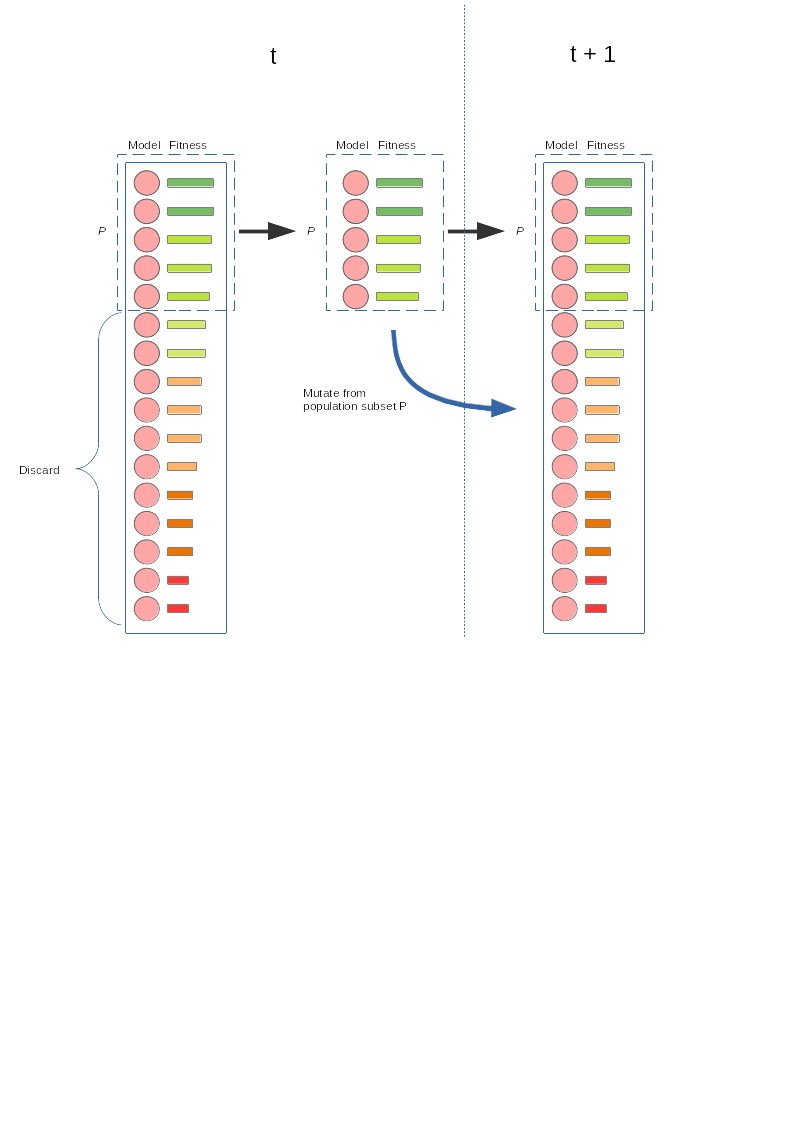
\includegraphics[trim= 100 450 100 0 ,scale=0.30]{Elite.png}


		\caption{Elitist selection where the population is subset down to a factor \text{P} from which the next generation is mutated. This form of selection is often considered naive and can lead to early convergence when used exclusively for selection.}
		\label{fig:GAX}


	\end{figure}


	A variant of tournament selection was used by \cite{42}, in which the population is selected against based upon the “age” of the network. This approach was used to set a new SOTA, performing at scale on ImageNET. This method maintains a population of networks along with a list which retains the age of each network ranking each from oldest to youngest based on when they were added to the population, as shown in Figure \ref{fig:GA2}. At each iteration a sample is draw from the population and the highest performing model is used to generate a new network. This new network becomes the youngest in the population and replaces the oldest network which is removed.



	\begin{algorithm}[H]\label{alg:GA1}
		\caption{Tournament Selection Algorithm}

		\SetAlgoLined
		\KwData{Samples size S, number of iterations C}\
		

		\For {i = 1 to C}
		{

			\While { $\|sample\| < S$}
			{
				$sample \leftarrow$ \text{random element from $population$}\;	
			
			}

			$parent \leftarrow$ best evaluation score in $sample$\;
			\textit{offspring} $\leftarrow$	MUTATE$(parent)$\;	
			$population \leftarrow$ TRAINANDEVALUATE$(\text{\textit{offspring}})$\;
			remove worst evaluation score in $sample$ from $population$\;

		}
		\Return{best evaluation score in population}\;

		
	\end{algorithm}





	\begin{figure}[h]
	
		\centering 
		\includegraphics[trim= 100 750 100 0 ,scale=0.35]{aging.png}


		\caption{Ageing tournament selection. This method takes the same approach as tournament selection however, rather than discarding the lowest performing model in the sample, the oldest network on the right of the age array is discarded. This promotes exploration by preferring younger networks in the population, helping to reduce the chances of the system becoming stuck in a local maxima early in the search process. }
		\label{fig:GA2}


	\end{figure}

\newpage
	\subsection{Speciation}

		NeuroEvolution of Augmenting Topologies (NEAT) \cite{24} describes a framework for evolving neural networks which addresses many of the issues faced by GA, such as a formalised system for crossover, genetic encoding, the permutation problem and the protection of innovation (This is discussed in Section \ref{encoding}). While NEATs success is limited to smaller networks, however, there have been several extensions to NEAT, adapting it for larger, deeper networks \cite{44}\cite{25}.
		One of the important contributions of NEAT was the use of Speciation. This method is used as a way to protect innovation in evolutionary systems by dividing the population into species which compete internally rather than with the population at large. This protects innovation by allowing new solutions to be explored and reach maturity without having to compete with older, more optimised networks. In practice this creates a less greedy algorithm supporting a greater diversity of solutions and, in theory, improving performance on highly multi-modal fitness functions. 
		Models are divided into species based on genetic distance, \(\delta\). Equation \ref{eq:NEAT1} describes the process for finding the genetic distance. \textit{E} and \textit{D} refer to \textit{Excess} and \textit{Disjointed} genes respectively, which is a component of the NEAT encoding system which is explained in Section \ref{crossover}. These are connections which are not common to both of the networks being compared, with \(C_1\) and \(C_2\) being weight hyperparameters that can be used adjust the impact of these attributes. \(\bar{w}\) denotes the difference in the parameter weights across common connections, with \(C_3\) again a coefficient controlling the importance. \textit(N) is simply a normalisation factor equal to the number of genes in the larger network. Using this metric, networks are placed into species based on a defined compatibility threshold, \(\delta_t\). At each iteration, a network is chosen at random from each species to represent the genotype of that species. New networks are then sequentially added to the first species with which \(\delta < \delta_t\), if there are no compatible species, a new species is created.

		\begin{equation}\label{eq:NEAT1}	\delta = \frac{C_1E}{N}+\frac{C_2D}{N}+C_3\bar{w}
		\end{equation}


		The number of offspring allocated to a species is based on the shared fitness of the species with respect to the entire population. Equation \ref{eq:NEAT2} describes the adjusted fitness, the sum of which is fitness for a species. This restricts one species from dominating the entire population. Within a sub-population, elitist selection is then performed before repopulating the species. 

		\begin{equation}\label{eq:NEAT2}	f_i' = \frac{f_i}{\sum_{j=1}^nsh(\delta(i,j))}
		\end{equation}

		\begin{equation}\label{eq:NEAT21} sh(\delta(i,j)) \begin{cases}
							1, & \text{if } \delta(i,j) < \delta_t\\\
							0, & \text{else}\end{cases} \end{equation}




	\subsection{Multi-Objective Selection}
		In multi-objective optimisation rather than maximising the solution according to a single criterion, there are a set of criterion \(f = \{f_i\}_{i=1}^N\), with respect to which the solution must be optimised. Often there is not a single solution which maximises all objective functions \(f_i\), this particularly true is cases where the \textit{f} contains functions which are in conflict rather than complimentary. In this scenario, there are often a range of Pareto optimal solutions with different characteristics.\cite{pareto}

		\subsubsection{Pareto Efficiency}

			A system is said to be Pareto efficient when no improvement can be made to any of the criterion \(f_i\) without causing a deterioration in at least one other criterion. This leads to a collection of solutions across the objective function space which are Pareto optimal, these are known as a Pareto set or Pareto front and are said to be non-dominated. Figure \ref{fig:GA3} shows an example of a Pareto front in two dimensional space.
			A solution is non-dominated when there is no solution which is better by one criterion and at least equal in all others. More formally this is given by equation \ref{eq:par1} for a two dimensional problem. These non-dominated solutions collectively form the Pareto set for a collection of solutions.


			\begin{equation}\label{eq:par1}
				(f_1(x) \geq f_1(\{x\}_{i=1}^N) ~\land~ f_2(x) > f_2(\{x\}_{i=1}^N))
				~\lor~
				(f_1(x) > f_1(\{x\}_{i=1}^N) ~\land~ f_2(x) \geq f_2(\{x\}_{i=1}^N))
			\end{equation}


			
			\begin{figure}[h]
			
				\centering 
				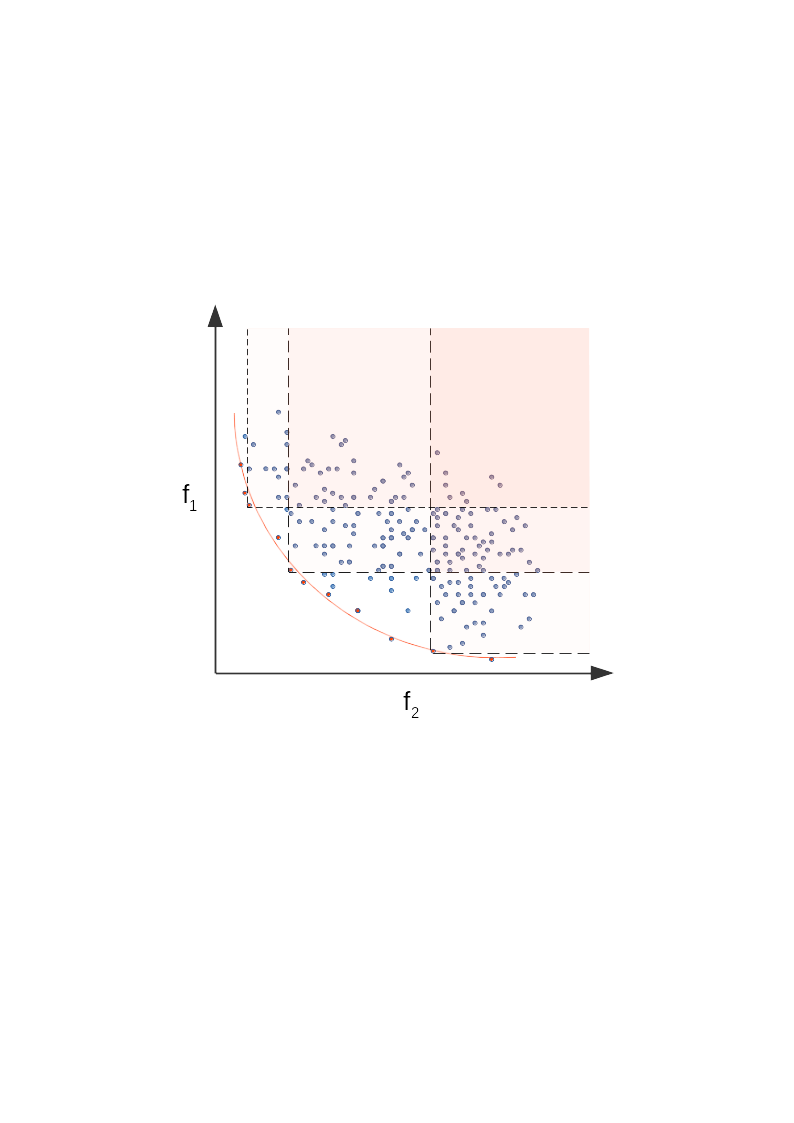
\includegraphics[trim= 250 380 250 210 ,scale=0.55]{pareto.png}


				\caption{Two dimensional optimisation problem. The red line denotes the Pareto front of the problem, with the red dots showing non-dominated, Pareto optimal solutions. The black dotted lines and shaded area show the area of objective function space which is dominated by the solutions at the origin of the line, note that this is only shown for a subset of the non-dominated points for clarity}
				\label{fig:GA3}


			\end{figure}










\newpage
		\subsubsection{LEMONADE and NSGA-Net}		

			A common secondary objective function in NAS or hyper-parameter optimisation after performance is model complexity. For applications in embedded systems or other computational limited environments, the complexity of the network can be an important factor. However, there are a number of metrics by which model complexity can be evaluated, such as, inference time, active network nodes, the number of model parameters or FLOPs (floating point calculations) in a forward pass of the network \cite{5}. 
			LEMONADE \cite{13} is multi-objective system which uses the model parameters as a measurement of complexity and leverage's the cheap evaluation cost in the selection process.

			This method uses Kernel Density Estimation (KDE) to build a distribution of networks with respect to complexity to select candidates for reproduction in sparse areas of the objective space (an example of KDE in a different application is shown in figure \ref{fig:tpe1}). The distribution generated by equation \ref{eq:mo1} is used to sample the initial set of offspring, where equation \ref{eq:mo2} is the normalisation constant. This process is then repeated sub-setting the offspring with equation \ref{eq:mo3}, where \(\hat{c}\) is again the normalisation constant similar to equation \ref{eq:mo2}. it is important to note that \(N\) refers to the subset of solutions that make up the Pareto front of non-dominated solutions.

			\begin{equation}\label{eq:mo1}
				P_p(N) = \frac{c}{P_{KDE}(f_{cheap}(N))}
			\end{equation}

			\begin{equation}\label{eq:mo2}
				c = \left(\sum_{N\in P}\frac{1}{P_{KDE}(f_{cheap}(N))}\right)^{-1}
			\end{equation}

			\begin{equation}\label{eq:mo3}
				P_p(N^c) = \frac{\hat{c}}{P_{KDE}(f_{cheap}(N^c))}
			\end{equation}


			NSGA-Net \cite{5} is another multi-objective optimisation system for NAS which is built upon NSGA-II algorithm\cite{42} for selection and incorporates Bayesian Optimisation methods. Rather than creating a distribution, NSGA-II iteratively allocates points into Pareto sets. This involves finding the initial set of non-dominated points assigning them to first layer of solutions and discounting them from the overall objective function space. This process is then repeated to fill out subsequent layers until there are no points remaining. These layers are then added to the next generation from the first layer down until the population limit is reached. 


		



	\subsection{Genetic Encoding}\label{encoding}



		Genetic encoding is a way of representing a network topology, parameters and hyper-parameters with the goal of allowing effective storage, crossover and transformation. Encoding methods can be broken down into two main categories, direct and indirect encoding.
		Indirect encoding refers to a system where rather than explicitly defining the structure of a network, a series of rules and structural motifs are defined from which the network is reconstructed. This allows for compact representations, often with repeating structures which has been shown to be successful in hand designed deep and convolutional networks \cite{DNN} \cite{CNN}. This type of encoding takes inspiration from biological systems with implementations based on composition pattern-producing networks (CPPNs) \cite{CPPN} having a foundation in embryonic development.\cite{NE}
		Direct encoding conversely, explicitly defines the attributes and topology of a system. This means the encoding (genotype) maps directly to the structure (phenotype). 

		The encoding scheme applied in NEAT is a direct encoding approach which maintains a list of connection and node genes. The connection gene contains the input node, output node, connection weight, innovation number and the enable bit. The node gene simply contains the innovation number and the type of node (i.e. input, output or hidden).


			\begin{figure}[h]
			
				\centering 
				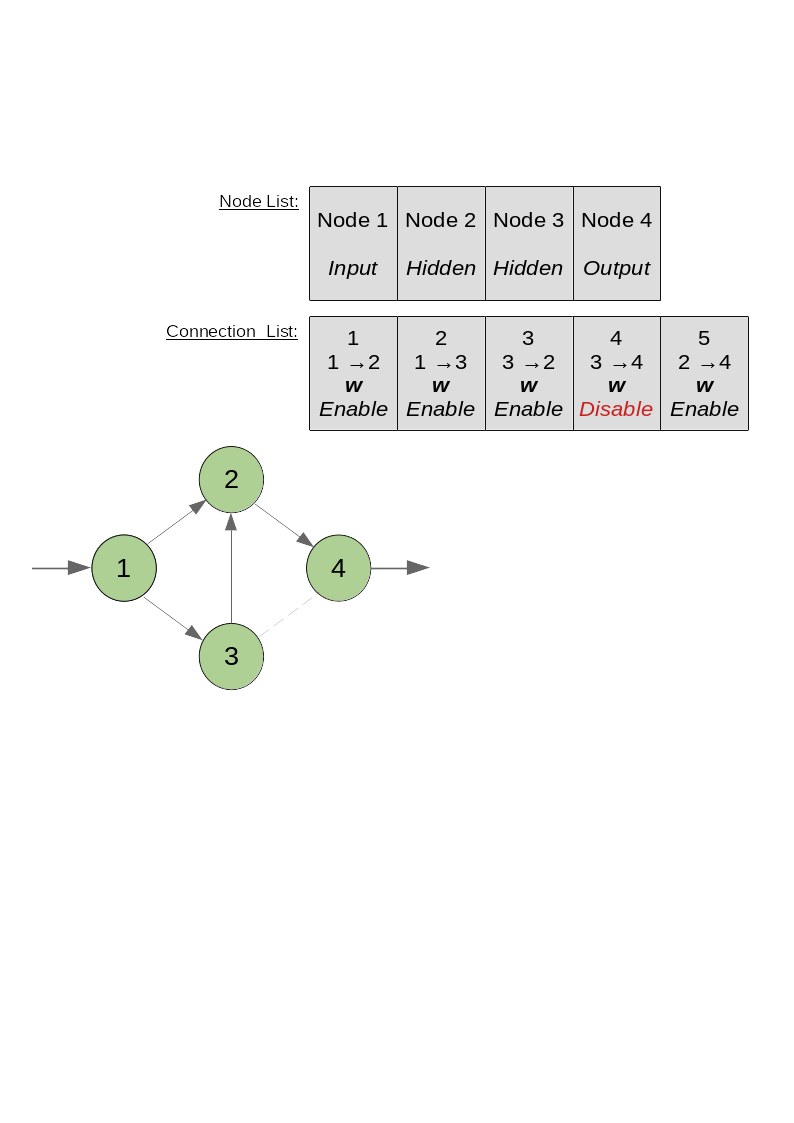
\includegraphics[trim= 250 380 250 110 ,scale=0.35]{NEAT.png}


				\caption{Example of the NEAT encoding scheme on a four node network. The connection list showing from top to bottom the innovation number, the input/output nodes, \textit{w} denoting the weight, and the enable bit. In this example the connection from node 3 to 4 is disabled, while this connect with no longer be active in the network, it remains important as a historical marker for computing the genetic distance and performing crossover. }
				\label{fig:GA3}


			\end{figure}

		A significant issue that is important to consider when designing a genetic encoding methods, in particular with respect to crossover, is the problem of competing conventions or the permutation problem\cite{38}\cite{24}. This occurs when there are multiple genomes which refer to the same phenotype. This can lead to loss of information, inefficient allocation of computational resources and irregularities during crossover operations. 

		NEAT makes use of an innovation number which is a core component to the overall NEAT system. The innovation number tracks the appearance of specific genes within the system. When a unique mutation occurs, it is allocated an innovation number, this number is incremented globally each time this occurs. Any subsequent occurrences of the same mutation are given the same innovation number. It is important to note that NEAT is not initialised randomly and rather all networks begin as a single connection between the input and output node, thus all networks effectively have a common ancestor and innovation numbers do not need to be assigned during initialisation.


	

	\subsection{Hierachical Model Design}

		CoDeepNEAT \cite{25} is an expansion to NEAT for use with deep neural networks. CoDeepNEAT is based on a bi-level optimisation approach to NAS and hyper-parameter optimisation problems, implementing a hierarchical approach in which “blueprints” and modules are evolved independently. This method moves away from the neuroevoluationary approach of NEAT for learning and instead uses gradient descent to optimise the weights of the model.

		A blueprint in this context is a graph of nodes which can be considered similar to the genotypes in NEAT. However, the nodes are replaced with smaller DNNs referred to as modules. These are combined together to produce a full network for evaluations. The fitness score of a network is applied to both the blueprint and the modules, with the module score being an average of all the networks which contained the blueprint. These two components are evolved independently as separate populations. This method was also applied to LSTM networks, where it was able to produce an LSTM variant using skip connections, which outperform the standard LSTM cell.


		Another similar approach was introduced in \cite{4} used a nested system for NAS which is similar to the method of CoDeepNEAT and employs an N-level hierarchy rather than a bi-level hierarchy. In this system, primitive operations (i.e. convolutional cells, linear cells, etc) are considered level one. Level two representations are a set of graph structures combining these lower level cells. These second level representations are then combined replacing the nodes in a graph to create higher level representation. Importantly, this method does not rebuild networks for each evaluation as is done in CoDeepNEAT, rather the networks are mutated in a more traditional process. The process was also able to achieve competitive results via a random search of this architecture space, implying that  the representation and design of the search space may have played a major role in the methods success.  


	\subsection{Crossover}\label{crossover}

		Crossover is the recombination of two successful networks into a “child” network which is used in certain GA approaches to NAS. \cite{3}\cite{24}\cite{5} This can be implemented through a wide variety of mechanisms based on the network encoding method which is used. Ablation tests on NEAT showed that while crossover can result in an overall improvement if carried out correctly, it was less significant that other aspects such as speciation \cite{5}\cite{24}. Figure \ref{fig:NEAT2} shows an example of crossover in NEAT. In this process genes are classified as \textit{Common}, \textit{Disjointed} or \textit{Excess}. Genes common to both parents are selected between randomly, whereas disjointed or excess genes are selected from the fittest parent. \textit{Disjointed} refers to genes which are unique to one parent but occur before the most recent innovation in the other parent, this implies less shared history between the genotypes. \textit{Excess} genes are unique to one parent but occur after the last innovation in the other parent.



		\begin{figure}[h]
		
			\centering 
			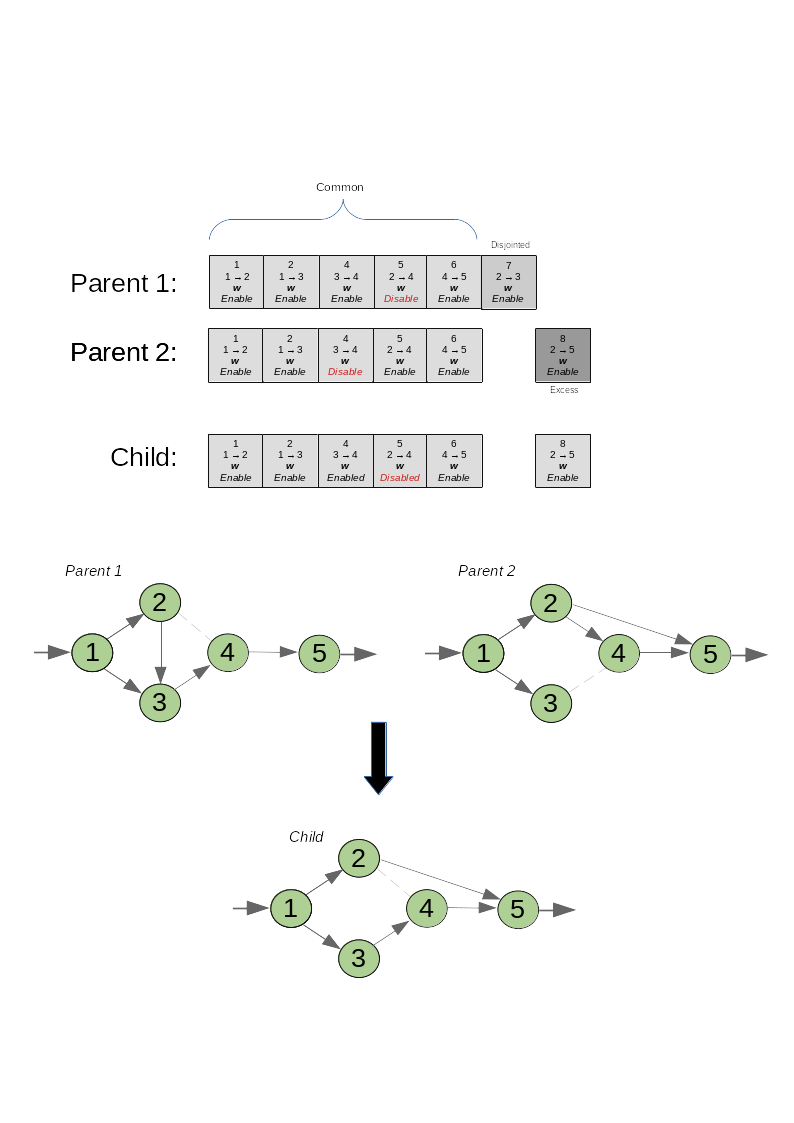
\includegraphics[trim= 250 120 250 210 ,scale=0.4]{NEAT2.png}


			\caption{Example of the crossover in NEAT. }
			\label{fig:NEAT2}


		\end{figure}



	\subsection{Mutation}

		Mutation is evolutionary systems is the process of perturbing or transforming some parameter or structure of a phenotype, generally without a pre-guided directive. This process must manage the balance between innovation, which is required to find new solutions and maintain diversity in the population, and preserving the internal functions and transforms of the model with which it achieved success. For numerical, continuous hyper-parameters a common approach is to permute the value according to a Gaussian distribution. For discrete variables it is common to employ bit-flipping \cite{25,39}. Topological mutation is generally implemented via a set of operations which can be applied to the network, although bit-flipping can be used in binary encoded implementations\cite{5}. The NEAT style mutation operators involve adding either a connection or a node to the network. In this case a node is added by disabling the connection where the node is to be placed, adding the node and two connections to the genotype, the first new connection having a weight equal to one, the second having the weighting of the old, now disabled connection. While the implementation differ most architecture mutations follow a similar procedure, having a operation which randomly selects a node or connection, then removes, adds or changes the operation of that component. These system commonly employ a bank of operations from which a new operation can be selected \cite{42,4}.
		\par
		A similar approach which takes a slightly different direction is the use of \textit{Network Morphisms} as described in LEMONADE. These are again transforms which are applied to the network, however, the goal of the operation is to deepen or wider the network while preserving the network function. A network morphism is a transform T, on a network N, which satisfies equation \ref{eq:mrp1} for \(x \in X\). This allows for the topology of the network to be expanded while maintaining the performance of the network. An example of this would be the addition of a layer to a network which is initialised to the identity function.
	
		\begin{equation}\label{eq:mrp1}
			N^w(x) = (TN)^w(x)
		\end{equation}

		This type of network transform has an obvious advantage for the efficient use of weight inheritance also know as Lamarckian Inheritance. This process has similarities with some neuroevolutionary approaches, as the network weights are maintained through the process of mutation and the generation of offspring. This be considered a form of warm-starting as networks are effectively pre-trained with their previous structure.   

		Another approach to weight inheritance is Population Based Training (PBT) introduced by \cite{39}. This is a GA which takes inspiration from bandit approaches to hyper-parameter optimisation. This was able to outperform human tuned networks on reinforcement learning and imagine classification tasks.
		\par
		This is a system for hyper-parameter optimisation which utilizes a variant of the  successive-halving\cite{SH} method used in HyperBand (see Sec 4.1) for early-stopping, A portion of the population abandon their search and copy the structure, hyper-parameters and weights of high performing networks. The hyper-parameters of this new replicated network are then mutated randomly to allow for more thorough examination of lucrative search spaces. This method of exploiting successful networks produces a schedule of hyper-parameters which change over the course of the training process rather than a static set. While this does offer the potential for a more dynamic training system, the size of the search space is increased dramatically as the number of hyper-parameter schedules is combinatorially larger than the original number of hyper-parameter sets.


\newpage

\section {Bayesian Optimisation}

	Bayesian Optimisation (BO) methods for hyper-parameter optimisation have become popular over the last decade due to the SOTA performance they can produce \cite{32} \cite{20}. One of the core weaknesses of many BO implementations is the lack of scalability, with models such as Gaussian Processes computationally scaling cubically with observations. The objective of BO and Sequential Model-Based Optimisation (SMBO) in general, in the context of hyper-parameter optimisation, can be described as trying to find \(x^* = argmin~ f(x)\) where \(x \in X\) and \(X \subseteq \mathbf{R} ^k\), \textit{X} is a bounded and compact region and \textit{k} is the dimensionality of the search space in our case the number of hyper-parameters. These methods assume correlation between observations and endeavour to use all of the available information to produce useful points for evaluating, \textit{x}, by exploiting a model constructed based upon a set of function query-observations pairs \( D = \{(x_n,y_n)\}_{n=1}^N\) where \(y_n \sim \mathcal{N}(f(x), \sigma_n^2) \).




	\subsection{Posterior Model}

		A posterior model uses the observation history \textit{D} often in combination with some prior to make estimation about the function \textit{f}. These models generally model the value of \textit{f} across the input space, either directly or indirectly, while also having some measure of uncertainty.




		\subsubsection{Gaussian Process}

			The most common model used in hyper-parameter optimisation is a Gaussian Process (GP)\cite{17}. The Gaussian process is non-parametric model which is widely used due to its flexibility and simplicity, allowing many common acquisition functions to be described in a closed form, while having a well calibrated measure of uncertainty. A GP can be considered a generalisation of a multivariate Gaussian distribution to any finite number of variables. In our case this denotes all possible values within the bounded region \textit{X}. A Gaussian process is fully defined, analogously to a Gaussian distribution, by a mean function, \(m(x)\) and covariance function \(K(x,x')\) shown in equation \ref{eq:gp1.1}. It is common to use \(m(x) = 0\) as the Gaussian process is generally robust to an arbitrary mean given sufficient data, which gives an equation for the GP as \ref{eq:gp1.2}.

			\begin{equation}\label{eq:gp1.1}f(x) \sim  \mathcal{N}(m(x) , K(x,x'))\end{equation}
			\begin{equation}\label{eq:gp1.2}f(x) \sim  \mathcal{N}(0 , K(x,x'))\end{equation}

			The covariance function or kernel function is used to generate the covariance matrices in a GP. The kernel is responsible for how both the prior and posterior are expressed. The most commonly used kernel function is the \textit{Squared Exponential Kernel}, given in equation \ref{eq:sek}. The covariance between two points is a function of their separation scaled by the hyper-parameter \textit{l}. 

			\begin{equation} \label{eq:sek} K(x,x') = \sigma^2 exp\left(-\frac{\mathopen|x - x'\mathclose|^2}{2l^2}\right)\end{equation}

			\begin{equation} \label{eq:ncov} K(x,x') = \sigma^2 exp\left(\sum_{i=1}^k-\frac{\mathopen|x_i - x_i'\mathclose|^2}{2l_i^2}\right)\end{equation}

			\begin{equation}\label{eq:sigy} \Sigma(x,x') = K(x,x') + I \sigma_y \end{equation}


			 Equation \ref{eq:ncov} shows the kernel function extended to multidimensional problem. for k dimensions there are k+3 hyper-parameters. \textit{l} is the scale length or the horizontal scaling, effectively how quickly the correlation between two points decays for each dimension. \(\sigma\) is the vertical scaling. \(\sigma_y\), shown in equation \ref{eq:sigy}, is a representation of noise in the evaluations, this maintains some uncertainty around evaluation points.  In hyper-parameter optimisation and other applications with noisy evaluations, Gaussian noise is added to the covariance matrix to avoid over-fitting. These hyper-parameters have a significant effect of the expression of the model and can be key to the final result, in particular \textit{l}. Because of this, these settings are normally dealt with automatically rather than hand tuned. One approach used in \cite{17} is to integrate over the hyper-parameters using Monte Carlo estimates, however this can be computationally expensive. Another common approach is to use a marginal likelihood estimates and optimise these settings via gradient descent.

 


			\begin{equation}\label{eq:gp1} p(f|\theta,D) = \mathcal{GP}(0,K(x,x'))\end{equation}

			\begin{equation}\label{eq:gp2} p(y|\theta,D) = \mathcal{GP}(0,K(x,x') + I\sigma_y)\end{equation}


 			Equations \ref{eq:gp1} and \ref{eq:gp2} show a definition of Gaussian processes over an noiseless and noisy function respectively. For a point of interested, y(x'), the Gaussian process can be considered a joint distribution over the y(x') and the query observation pair history \textit{D}. Using the marginalisation property of gaussians this can be restructured as equation \ref{eq:gp4}. An estimate of \textit{y} at \textit{x'} is simply \textit{y(x')} conditioned on \textit{y(\textbf{x})}, shown in equation \ref{eq:gp4.1}

			\begin{equation}
			\label{eq:gp4} p(y(\bm{x}),y(x')) \sim \mathcal{N} \left(\begin{pmatrix}
			0\\
			0
			\end{pmatrix}
			\begin{pmatrix} K(\bm{x} , \bm{x}) & K(\bm{x},x')\\
							K(\bm{x},x')^T &  K(x',x')
			\end{pmatrix}\right)\end{equation}

			%\begin{equation}\label{eq:inv} p(y(x')|y(\bm{x})) = \frac{p(\bm{x},x')}{p(\bm{x})} \sim  \mathcal{N} (K(\bm{x},x')K(\bm{x},\bm{x}})^{-1}y(\bm{x}),K(x',x') - K(\bm{x},x')K(\bm{x},\bm{x}})^{-1}K(\bm{x},x')^T) \end{equation}


			\begin{equation}\label{eq:gp4.1}p(y(x')|y(\bm{x})) = \frac{p(\bm{x},x')}{p(\bm{x})} \sim  \mathcal{N} (\mu',\sigma') \end{equation}



			\begin{equation}\label{eq:gp4.2}\mu' = K(\bm{x},x')K(\bm{x},\bm{x})^{-1}y(\bm{x})\end{equation}
			\begin{equation} \label{eq:gp5}\sigma' = K(x',x') - K(\bm{x},x')K(\bm{x},\bm{x})^{-1}K(\bm{x},x')^T \end{equation}



			Equations \ref{eq:gp4.2} and \ref{eq:gp5} show the computational issue with Gaussian processes, the inversion of the posterior covariance matrix, \(K(\bm{x},\bm{x})\). This is a \((N,N)\) matrix which means the computational complexity scales cubically \(O(n^3)\) with the number of observations. This issues is further exacerbated in high dimensional search spaces causing GPs to become intractable on large scale, high dimensional problems. Due to the expensive function evaluations in hyper-parameter optimisation, these computational expenses have, until recently, been easily justifiable. However, with the increasing ubiquity of parallel and cloud computing in ML, this limitation has lead to interest in other, more scalable models.


		\subsubsection{Tree-Structured Parzen Estimator}

			The Tree-Structured Parzen Estimator (TPE) is a model introduced by \cite{20} based on Parzen Window Density or Kernel Density estimation. This method was also claimed to outperform both random and GP based Bayesian hyper-parameter optimisation on the MNIST data-set \cite{20}. BOHB\cite{32} has more recently used a similar method to great success, leading to its use as the underlying system in the popular Auto-ML tool “HyBandSter” \cite{34}.
			TPE takes an alternative approach to the GP, modelling \(p(x|y)\) and \(p(y)\) rather than \(p(y|x)\) directly. This approach makes use of Kernel Density Estimation (KDE) to build two distribution of hyper-parameter settings which is shown in Figure \ref{fig:tpe1}. Equation \ref{eq:TPE} describes the criterion for discriminating between evaluations for division into either \(l(x)\) or \(g(x)\) in a maximization problem. Here \(y*\) is set to be some quantile of the evaluations \(y\) rather than the maximum, this creates two probability distributions one of high performing hyper-parameter combinations and another of lower performing combinations. 

			\begin{equation}\label{eq:TPE} p(x|y) \begin{cases}
									l(x), & \text{if } y>y*\\
									g(x), & \text{if } y\leq y*\end{cases} \end{equation}

			\begin{figure}[h]

			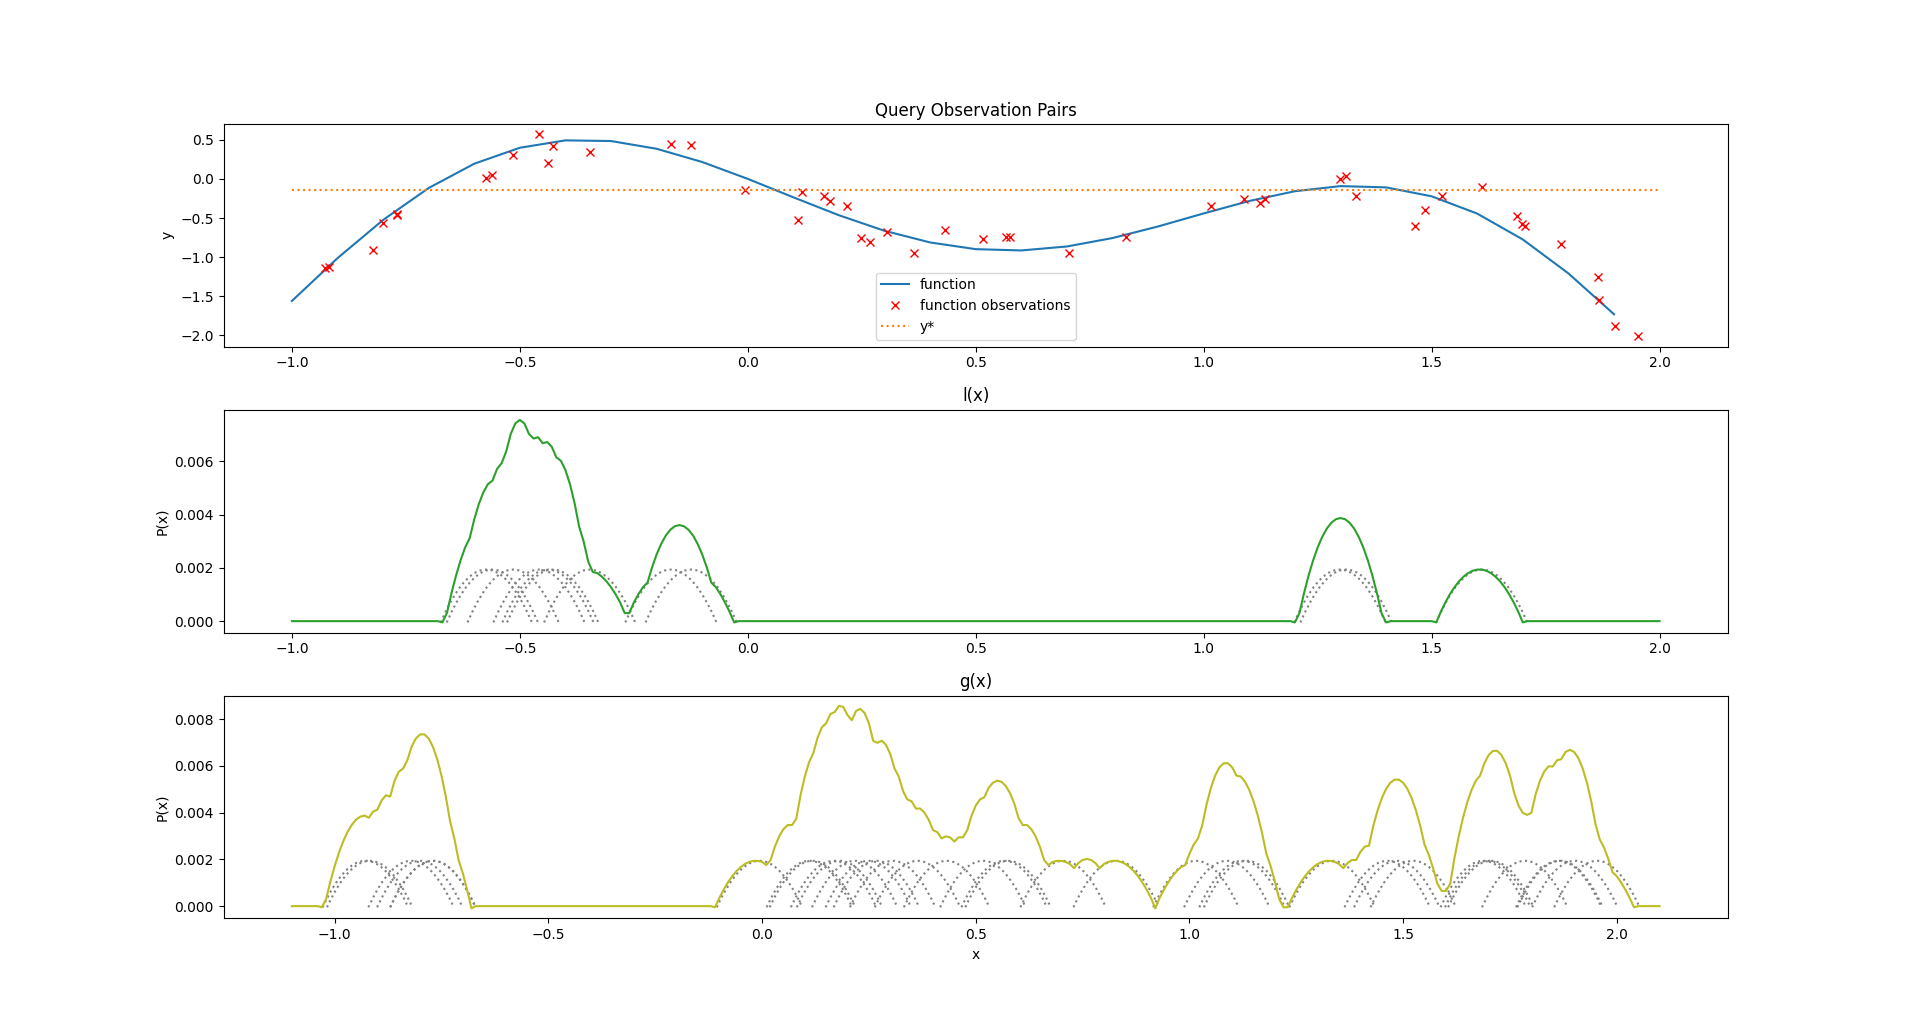
\includegraphics[trim=20 0 0 0 ,scale=0.25]{TPE1.png}

			\caption{Example of the distributions created by KDE during TPE on a 1-dimensional maximisation problem. Top shows noisy observations of a function with y* set so that l(x) contains the upper quartile of evaluation scores. The middle and lower plots show KDE with a Gaussian kernel shown by the dotted lines.}
			\label{fig:tpe1}
			\end{figure}
			Query point acquisition which is discussed in section \ref{AF}, is also simple with TPE. As shown in equation \ref{eq:TPE2}, the ratio of l(x) over g(x) is maximised, this was shown to be equivalent to maximizing EI \cite{20} (Section \ref{EI} ).

			\begin{equation}\label{eq:TPE2} x_{next} = argmax \frac{l(x)}{g(x)}\end{equation}


		\subsubsection{Bayesian Neural Networks}

			Another method for modelling the distribution over a function is with the use of a Bayesian neural network. DNGO \cite{22} is an implementation of this that uses a Deep Neural Network in combination with a Bayesian linear regressor to create an adaptive basis regression to model the posterior. This approach has the advantage of scaling linearly, in terms of computation, with the number of observations rather than cubically as with a GP. This method was able to achieve parity with SOTA in hyper-parameter optimisation on CIFAR-10. BOHAMIANN \cite{40} is another implementation of Bayesian neural networks which was able to out perform DNGO on a number of hyper-parameter optimisation tasks while supporting native parallelisation. 
			\par
			One significant issue with neural network based BO methods is the reliance of these techniques on well tuned hyper-parameters of their own to achieve optimal performance. This resulted in DNGO applying the more robust hyper-parameter optimisation system \textit{spearmint} (based on \cite{20}) to the system to optimise its own hyper-parameters.




	\subsection {Acquisition Function} \label{AF}

		The acquisition function is used in BO to select the next query point in hyper-parameter space at which to evaluate, \(x_{next}\), based on the posterior model. This can be considered the criterion against which the latent value of a point in the search space is evaluated. The exploit/explore problem is managed by this component of the system, balancing the use of known high value regions with information gain from areas with large uncertainty. Parallelisation is another important design feature of the acquisition function. Many popular and effective methods are natively sequential and therefore require modification or extension to accommodate parallel query point acquisition. There are asynchronous implementations used as a solution to this problem, which commonly involve updating the posterior model as a worker completes an evaluation, producing a new query point from the updated posterior model and re-dispatching the worker. \cite{26}\cite{27}\cite{20}



		\subsubsection{Expected Improvement}\label{EI}

			The most common of acquisition function, in particular when paired with a GP, is Expected Improvement (EI) due to the fact it is considered robust for most problems and does not require complex hyper-parameter tuning of its own. Equation \ref{eq:ei1} defines EI, which can be described as the expectation that a query point \(x\) will improve upon the current best evaluation in the next step, leading to a greedy choice of query points. Equation \ref{eq:ei2} shows how EI can be evaluated in closed form under a GP. From this the framing of the exploration/exploitation problem in terms of \(\Delta_n\) (predicted mean - current best estimate) and predicted variance \(\sigma_n\) can be seen. EI is high when \(\Delta_n\) is large and largest when both  \(\Delta_n\) and \(\sigma_n\) are high, with the former having a much larger effect. The exploration coefficient, \(\xi\), is shown in equation \ref{eq:ei3}. This hyper-parameter limits the greediness of the criterion by devaluing the posterior mean relative to uncertainty, promoting exploration.

			 

			\begin{equation}\label{eq:ei1} EI_n(x) = \mathbf{E} ~max(f(x) -f(x*),0)\end{equation}

			\begin{equation}\label{eq:ei2} EI_n(x) = [\Delta_n(x)]^+ \sigma_n(x)\varphi\left(\frac{\Delta_n(x)}{\sigma_n(x)}\right)  - |\Delta_n(x)| \Phi\left(-\frac{|\Delta_n(x)|}{\sigma_n(x)}\right)\end{equation}

			\begin{equation}\label{eq:ei3}\Delta_n(x) = (\mu(x) - f(x*) - \xi) \end{equation}


			Maximizing EI can be done with a number of approaches. One simplistic approach is simply to perform a grid search over the function. However, one of the beneficial attributes of EI under a GP is the often at least ones differentiable (conditional on the kernel) allowing for gradient descent to be used. it is important to note that EI tends to produce a function which is highly multi-modal, this means in practice gradient descent is restarted from a number of random locations in-order to find the global optimum. Figure \ref{fig:EI1} shows that even in simple problems EI can be multi-modal in nature.
				

			\begin{figure}[h]

			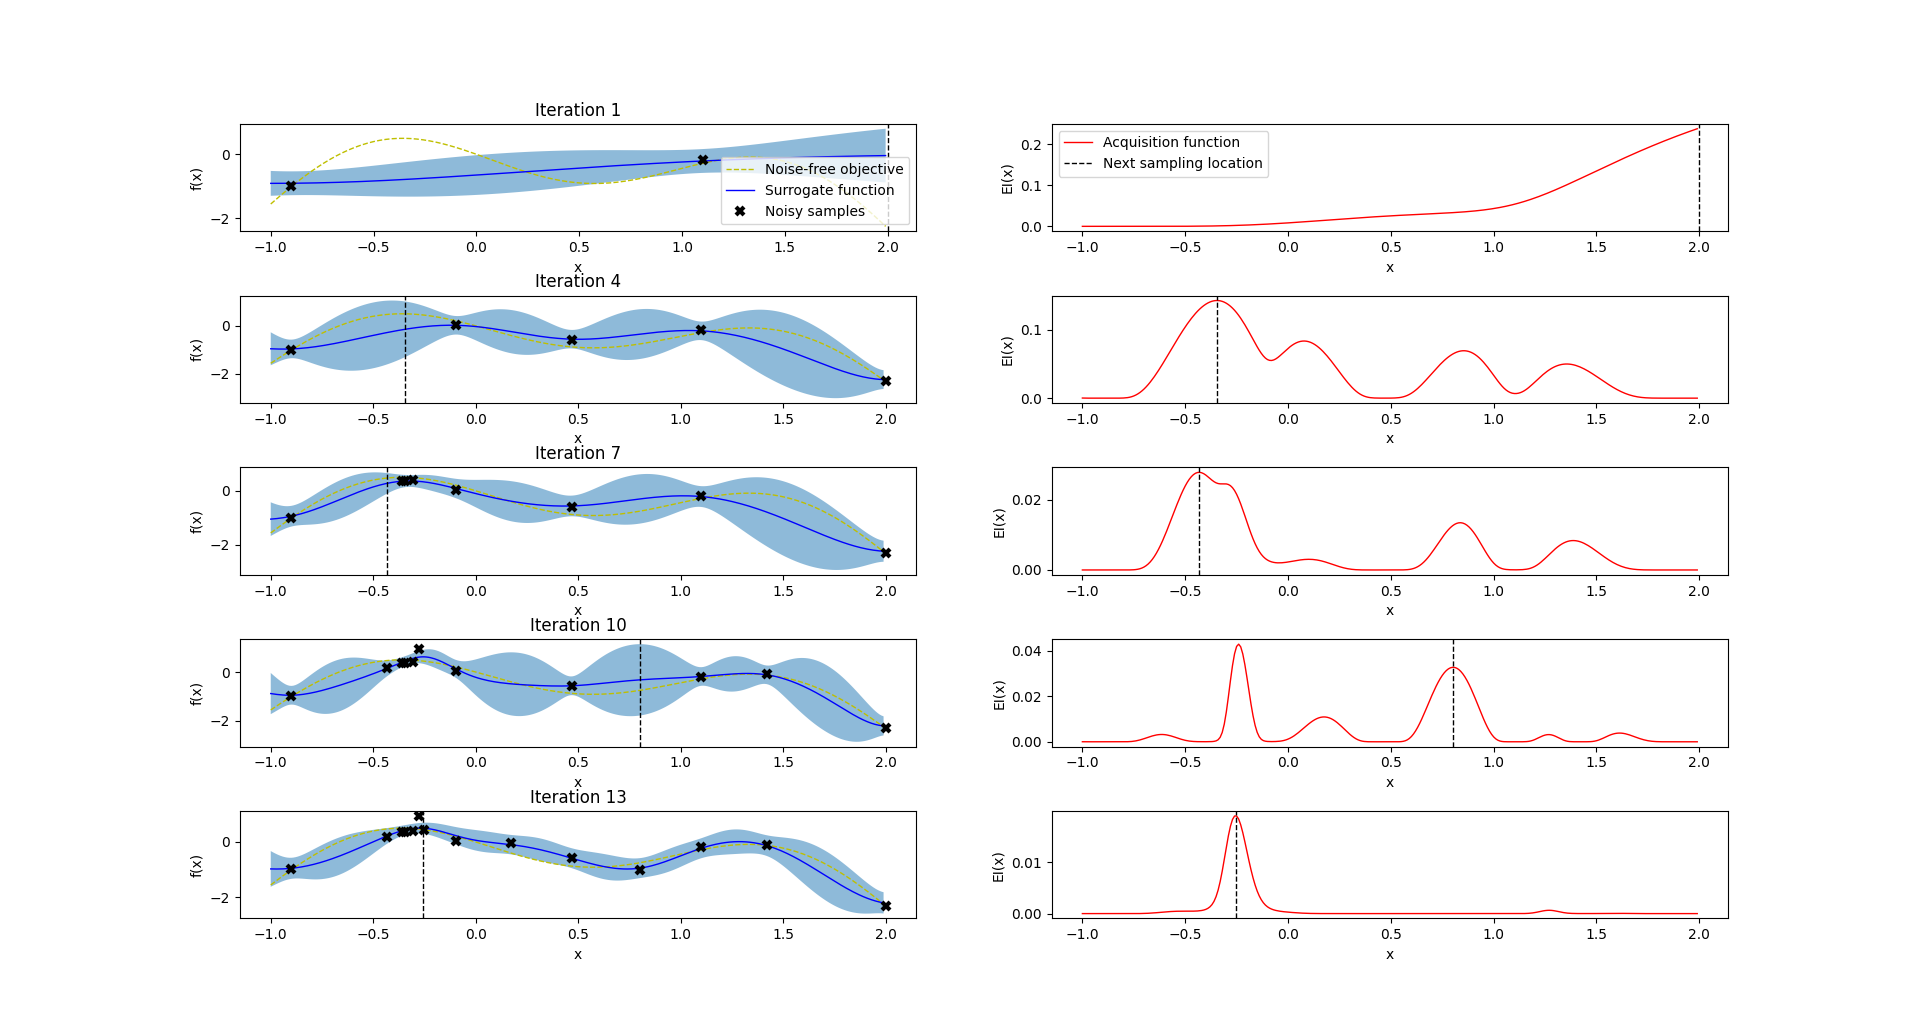
\includegraphics[trim=20 0 0 0 ,scale=0.25]{EIsimp.png}

			\caption{
			Expected improvement optimising a simple one-dimensional problem over a GP for 13 iterations. Left shows the Gaussian process modelling the posterior. Right shows the value curve at selected iterations under the EI criterion.
			}
			\label{fig:EI1}

			\end{figure}

			\subsubsection{EI-MCMC}\label{EI-MCMC}

			EI-MCMC is an extension of this function which allows for parallelisation based on Monte Carlo Markov Chain estimates of the acquisition function \cite{17}. In a case where there are a set of \textit{J} points being currently evaluated in parallel, EI cannot simply be re-evaluated on the same posterior as it would produce a redundant evaluation. This approach makes a Monty Carlo estimates via slice sampling at the ongoing evaluation points \({\{x\}}_{j=1}^J\) of the evaluation outcomes, \(\{y\}_{j=1}^J\). One set of these outcomes is referred to as a 'fantasy'. Optimally, EI would be computed across all possible values for \(\{y\}_{j=1}^J\) and the next point selected by integrating over the EI outcomes. In practice this is calculated over a finite number of fantasies with the \(x_{next}\) being the argument maximizing the result of integrating over the acquisition function outputs, described in \ref{eq:EI4}.

			\begin{equation}\label{eq:EI4} x_{next} = argmax~ \widehat{EI}(x; D, \theta,\{x_j\})\end{equation}


		\subsubsection{Upper Confidence Bound (UCB)}
			Upper Confidence Bound (UCB) is an approach to query point acquisition which is optimistic towards uncertainty. This, ideally, results in a system which is less greedy, and consequently less likely to become trapped in local optima. Simply attempting to maximizing the information gain at each iteration, a greedy approximation of which is given by \ref{eq:UCB2}, gives a criterion for quickly reducing the global uncertainty in the posterior. In practice however, this is not efficient as not only will it produce query points where \(\mu(x)\) is known to be poor, but it fails to utilize function evaluations, \(y(x)\), entirely. This observation is an important aspect of GP-BUCB, discussed in Section \ref{BUCB}. Equation \ref{eq:UCB1} describes GP-UCB \cite{GP-UCB}, which rather than attempting to reduce across the entire function, attempts to reduce uncertainty in the proximity of the maxima. \(B_n\) is a constant which is used to scale the dependence on the uncertainty. UCB more-so than other acquisition functions requires an accurately calibrated measure of uncertainty which encapsulates \(f\) entirely.



			\begin{equation}\label{eq:UCB2} x_t = argmax ~\sigma_{t-1}(x) \end{equation}


			\begin{equation}\label{eq:UCB1} UBC(x) = \mu(x) + B_n\sigma(x) \end{equation}




		\subsubsection{Batched Upper Confidence Bound (BUCB)}\label{BUCB}

		GP-BUCB is an extension to UCB introduced by \cite{GP-BUCB} which allows for parallel query point acquisition. This approach builds on the observation from the previous section on equation \ref{eq:UCB2} that the variance of the posterior model is independent of the function evaluation and dependant only on the evaluation location. This is shown in equation \ref{eq:gp5}, however, this also highlights the computational bottleneck of this process as the posterior covariance matrix inversion is still required. In order to be feasible this required a surrogate method for calculating the variance. Another issue is over confidence of the posterior model when the variance has been updated with unevaluated queries, as UCB relies heavily on this uncertainty. One proposed solution to this is to use highly conservative confidence bounds to ensure that the true function is captured.\cite{GP-BUCB}




		\subsubsection{Local Penalisation}

			One intuitive solution to the problem of parallelisation is the application of local penalization to an acquisition function in order to create batches of query points as shown in \cite{37}. This approach iteratively applies a penalty to the acquisition function directly for each query point in a batch. The goal of this method is to produce a set of query points which explore separate modes of the acquisition function. Algorithm \ref{alg:LP1} describes this process, where \(\varphi_j(x)\) is the local penalisation function and \(\widetilde{a_j}(x)\) is the transform of the acquisition function.
			
			\par \(~\)

			\begin{algorithm}[H]\label{alg:LP1}
			\caption{Local Penalisation for BO}
			\SetAlgoLined
			\KwData{observation history \(D = \{(x_n,y_n)\}_{n=1}^N\), batch size ~J}\
			\KwResult{\(B_J = \{x_0,...,x_J\}\)}\

		  	\(x_{next,0} = a(x)\)\;

		  	\(\widetilde{a_0}(x) = \leftarrow \widetilde{a}(x)\varphi_{0}(x)\)\;


			\For {j =1 to J}
			{
				\(\widetilde{a_j}(x) \leftarrow \widetilde{a}(x)\varphi_{j}(x)\)\;

			  	\(x_{next,j} = \widetilde{a_j}(x)\)\;

			}

			
			\end{algorithm}

			\par \(~\)

			However, this method can be consider as “doubly greedy” \cite{36} in cases where a greedy acquisition function is used as the basis for local penalisation.




		\subsubsection{Thompson Sampling}

			Thompson Sampling (TS) is one method that has been applied to the problem of BO Parallelisation\cite{26}\cite{27}. TS has performed well when compared with other parallel BO methods on a number of hyper-parameter optimisation tasks including the CIFAR-10 data-set. 
			Thompson sampling is an approach to the exploitation/exploration problem in which an assumption is made about the value of a variable based on a sample from a probability distribution. In the context of BO and more specifically in application under a GP, TS involves sampling across the posterior distribution to create a sample function, \(g\). The next query point can then simply be evaluated as \(x_{next} = argmax ~g(x)\). Figure \ref{fig:TS1}, shows an example of how TS can produce diverse sampling locations in parallel. Thompson Sampling was shown in \cite{27} to perform only marginally worse in parallel implementations, either synchronous or asynchronous, when compared with a sequential variation with the same number of total evaluations.



			\begin{figure}[h]	


			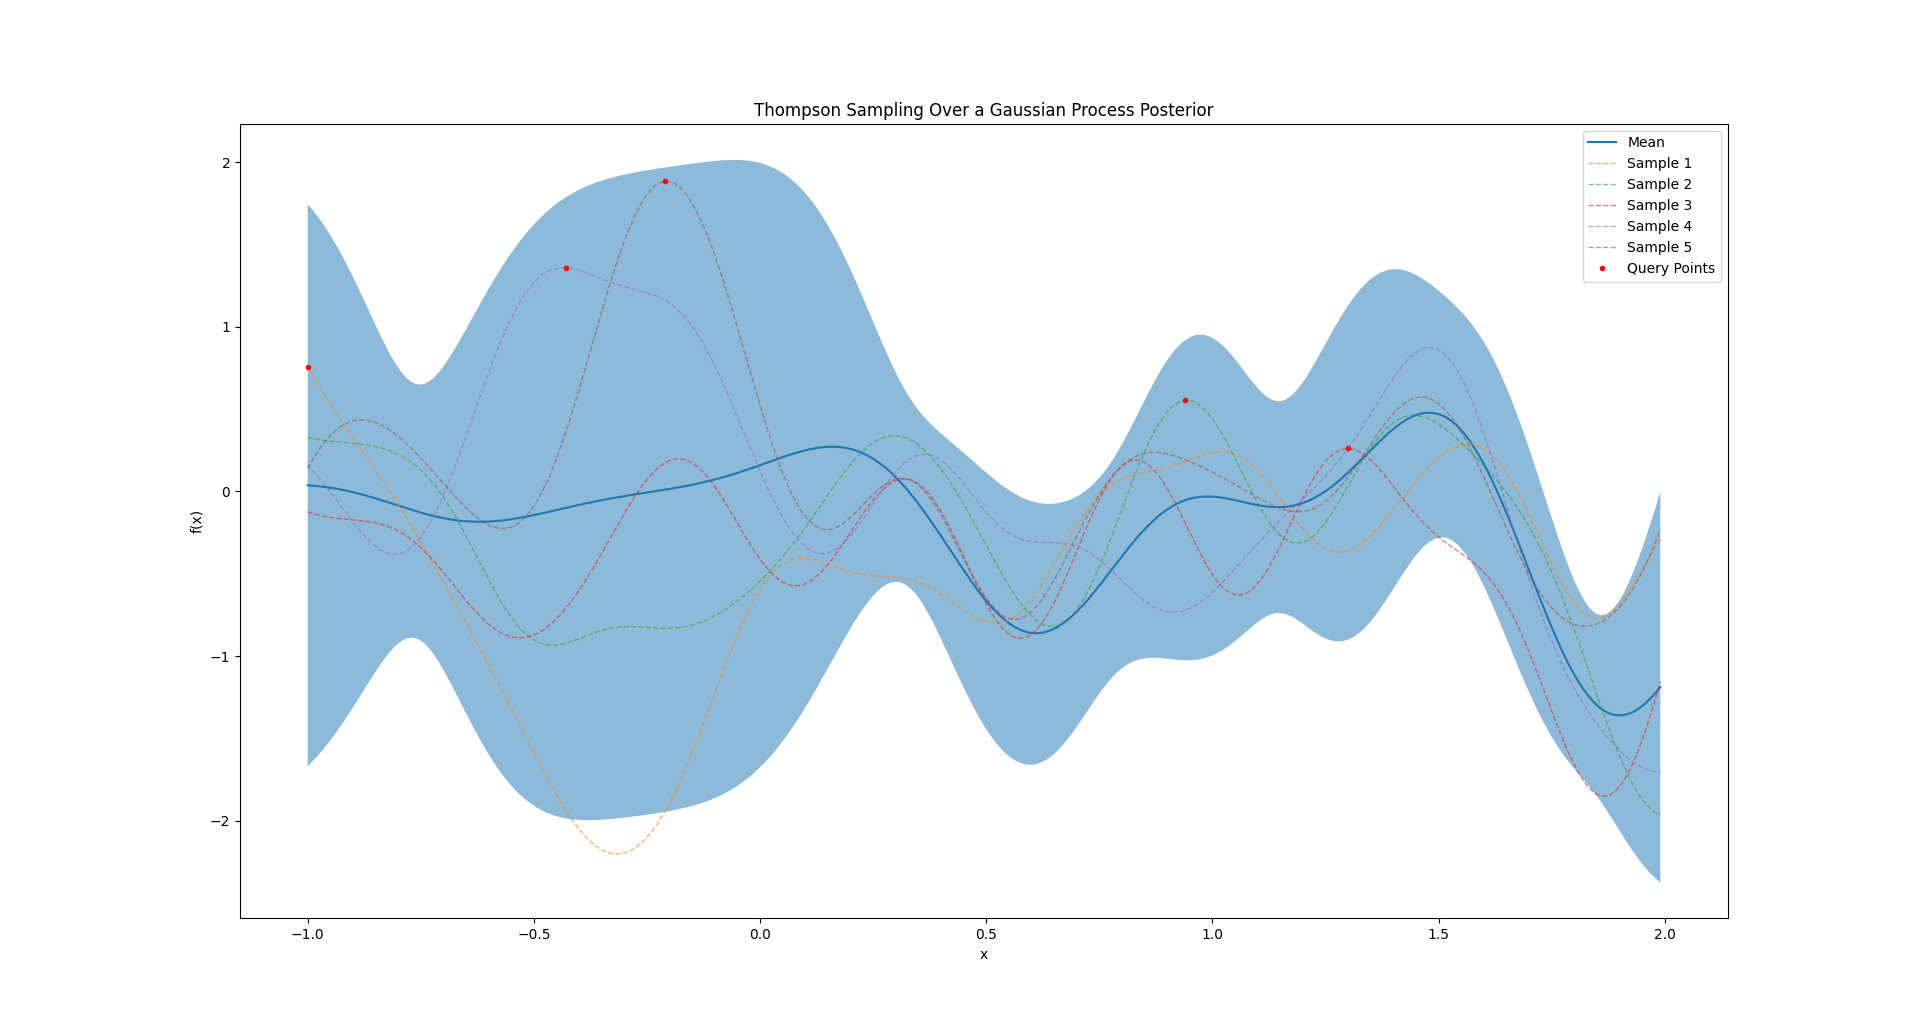
\includegraphics[trim=20 0 0 0 ,scale=0.25]{TS.png}

			\caption{Synchronise query point acquisition for a batch of five points with Thompson Sampling under a GP.}
			\label{fig:TS1}

			\end{figure}


			A similar approach which utilizes Thompson Sampling, AEGis, introduction by \cite{26}, combines this technique with periodic random selection of query points. This method was able to outperform other Parallel BO methods on synthetic function optimisation, however, it was unable to compete with vanilla TS on hyper-parameter optimisation tasks. When compared with TS, AEGiS also performed worse as the number of workers increased.


\newpage
\section {Many-Armed Bandit and Early-Stopping}



	The problem of hyper-parameter optimisation can also be framed as a many armed bandit problem. 
	A bandit problem describes a problem where an agent has a number of possible actions which yield a reward. Initially the association between an action and its reward is unknown to the agent. In a classic stochastic bandit problem, each action produces a reward randomly based on the probability distribution of reward linked to that specific action. The agent must therefore make a series of actions to gain information about reward associated with each action while also attempting to maximise the total reward. Figure \ref{fig:BP1}  shows an example of this type of problem. 

	\begin{figure}[h]\label{fig:BPI}
	
		\centering 
		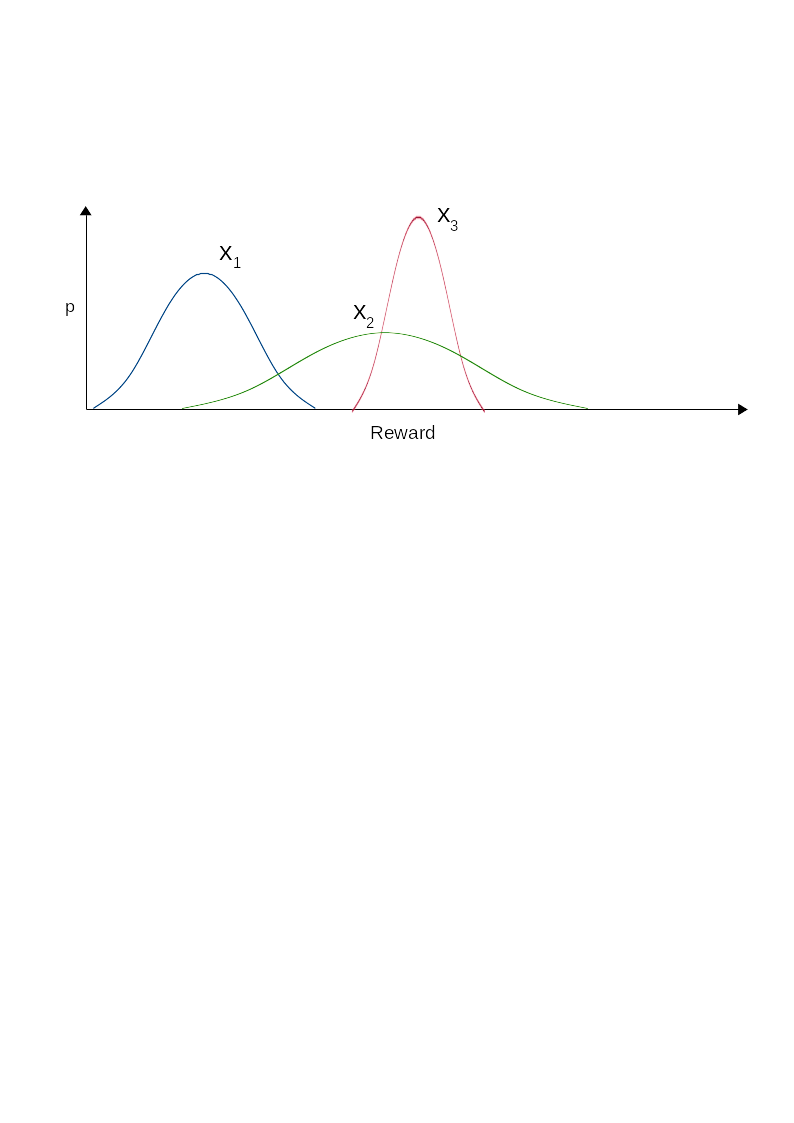
\includegraphics[trim= 100 650 100 100 ,scale=0.5]{BanditIntro.png}


		\caption{Bandit problem example with three actions denoted as \(x_1\),\(x_2\) and \(x_3\). Each of these actions has an probability curve over a range of reward values which represents an agents belief about the value of each action. In this case there is a much higher uncertainty in \(x_2\) than \(x_3\) which has a higher mean value. A highly greedy approach to this problem would lead to the exploitation of \(x_3\) rather than the exploration of \(x_2\), which may not the optimal solution.}



	\end{figure}


	\par

	Hyper-parameter optimisation can be considered a non-stochastic variant of this problem. In this case an action or 'pull' becomes a single, or collection of, training iterations with a set of hyper-parameters. The models cost function or loss on the validation data set becomes the associated reward.  In this application it is only the simple regret that is of interest rather than the cumulative regret as it is only the final recommendation which the search is evaluated on.


		\begin{equation}\label{eq:BP1}	l_{\theta,t} = \frac{1}{|VAL|} \sum_{i \in VAL} loss(f_{\theta,t}(x_i),y_i)\end{equation}



	Equation \ref{eq:BP1} describes the reward in this application, the cost function over the validation set. where \(f_{\theta,t}\) is the function modelled by the algorithm that is being optimised, after a number of training steps \(t\) and a set of hyper-parameters \(\theta\)


			\begin{figure}[h]
			
			\centering 
			\includegraphics[trim= 100 100 100 300 ,scale=0.45]{bandit.png}


			\caption{Four steps of the Successive Halving algorithm. }
			\label{fig:BP1}


			\end{figure}



	\subsection{Successive Halving}

	Successive Halving is an algorithm first introduced in \cite{SH0} for stochastic bandit problems and later adapted for the non-stochastic domain of hyper-parameter optimisation \cite{SH}. This technique has become the basis for much of the bandit style approaches to hyper-parameter optimisation. In this approach the set of possible actions is constrained to a randomly initialised set of hyper-parameter settings, \(S_0\).
	Each iteration of the algorithm has the set of models trained for a number of steps based on a budget, \(B\), and the number of models ,\(n\). after each training interval the models are evaluated according to \ref{eq:BP1}. The set of \(S_0\) is then subset to half its size based on this metric. Figure \ref{fig:BP1} shows an a series of iterations of Successive Halving which is more formally described in Algorithm \ref{alg:BP1}.


	\par
	

		\begin{algorithm}[H]\label{alg:BP1}
			\caption{Successive Halving for Hyper-parameter Optimisation}

			\SetAlgoLined
			\KwData{Initial Set of hyper-parameter settings \(S_0 = \{n\}\), budget B}\
			
			
			\KwResult{Final set containing single model, \(S_{k=log_2(n)}\)}\

			\For {\(k = \{1,2,...,log_2(n)\}\)}
				{

				\For {\(j  \in S_k\)}
					{
					\(Train S_{k,j} ~for~ \frac{B}{|S_k|log_2(n)} steps\)\;

					\(l_{k} = \{l_k,\frac{1}{|VAL|} \sum_{i \in VAL} loss(S_{j,k}(x_i),y_i)\}\) \;
					

					}


				\For {\(j_s,j_l \in S_k,l_k\)}
					{
					\If {\(j_l > median(l_k)\)}
						{

						\(S_{k+1} = \{S_{k+1},j_s\}\)\;

						}

			
			  		}
			
				}		
		\end{algorithm}



		This type of approach is also referred to as Early-Stopping and is based on the assumption that a partially trained models performance will be predictive of its final performance [32][47]. This assumption can, however, become strained in applications where the convergence time of models has a significant variance across the search space. One of the limitation of this type of solution, in particular when the initial set of models is seeded from a simple random search, is final performance with a large computational budget.  Sequential methods such as Bayesian Optimisation or Genetic Algorithms are often able to achieve better performance given a large enough budget. This has lead to the incorporation of bandit based strategies into Bayesian and Evolutionary techniques to improve the any-time performance as well as allowing for greater exploration, due to the increase in efficiency. \cite{32,34,39}  Asynchronous Successive Halving Algorithm (ASHA) \cite{34} is a more recent parallelisation technique for the Successive-Halving algorithm. This method has been shown to perform as well as or better than other techniques that incorporate early stopping such as PBT, BOHB and HyperBand on a variety of hyper-parameter optimisation and NAS benchmarks.



	\subsection{HyperBand}

		HyperBand \cite{HB} is an popular example of this strategy and has shown the effectiveness of this method, in particular with respect to any-time performance. HyperBand was able to achieve a reduction in training time of an order of magnitude over Bayesian methods while maintaining only a minor reduction in performance. HyperBand can be considered a resource allocation algorithm for Successive-Halving \cite{SH}, running as a meta layer around a series of Successive-Halving inner loops which are referred to as 'brackets'. This approach attacks the problem of balancing the resources budget \(B\), between the training time for each model \(r\), with the total number of models trained \(n\). Due to the variance of model convergence time between different algorithms or problem domains, this cannot be a static, fit all value. HyperBand effectively performs a grid search over values of n and r, running a sequence of tests for different values of n within a bounded range. 



		\begin{algorithm}[H]\label{alg:HB}
			\caption{HyperBand}

			\SetAlgoLined
			\KwData{R, \(\eta\)}\
			
			\Init{ \(s_{max} = \left[ log_\eta(R) \right] , B = (s_{max} +1)R\), Model evaluation scores l = \{\}}\



			\For {\(s = \{s_{max},s_{max}-1,...,0\}\)}
				{
				\(n = \left[ \frac{B}{R}\frac{\eta^s}{(s+1)} \right]\)\;

				\(r = R\eta^{-s}\)\;

				\(S_0 \leftarrow \text{randomly\_generate\_hyperparameter\_sets}(n)\)\;

				\(l \leftarrow SucessiveHalving*(S_0,r,\eta)\)\;

				}
			\Return{max(l)} 

		\end{algorithm}

		Algorithm \ref{alg:HB} describes HyperBand and its relation to Successive-Halving which is modified in this case to take a minimum amount of resources, \(r\) and \(\eta\) which denotes the factor by which the number of models is reduced by at each round. \(R\) and \(\eta\) are user defined hyper-parameters, with the former defining the maximum resources allocated to a single model between evaluations. The total number of brackets is defined by \(s_{max}\). 


\section{Reinforcement Learning}

	Reinforcement learning is an approach to NAS which became popular with the introduction of RL-NAS \cite{NAS-RL} which utilised a controller agent trained via reinforcement learning to generate model architectures for image classification and natural language processing problems. This approach was able to set a new state of the art in CIFAR-10, outperforming human hand-designed systems. Figure \ref{fig:RL} shows an example of the controller network. While this approach was able to achieve very strong performance, the computational budget required was extremely large, requiring 22,400 GPU days of training. 
 
	\begin{figure}[h]

			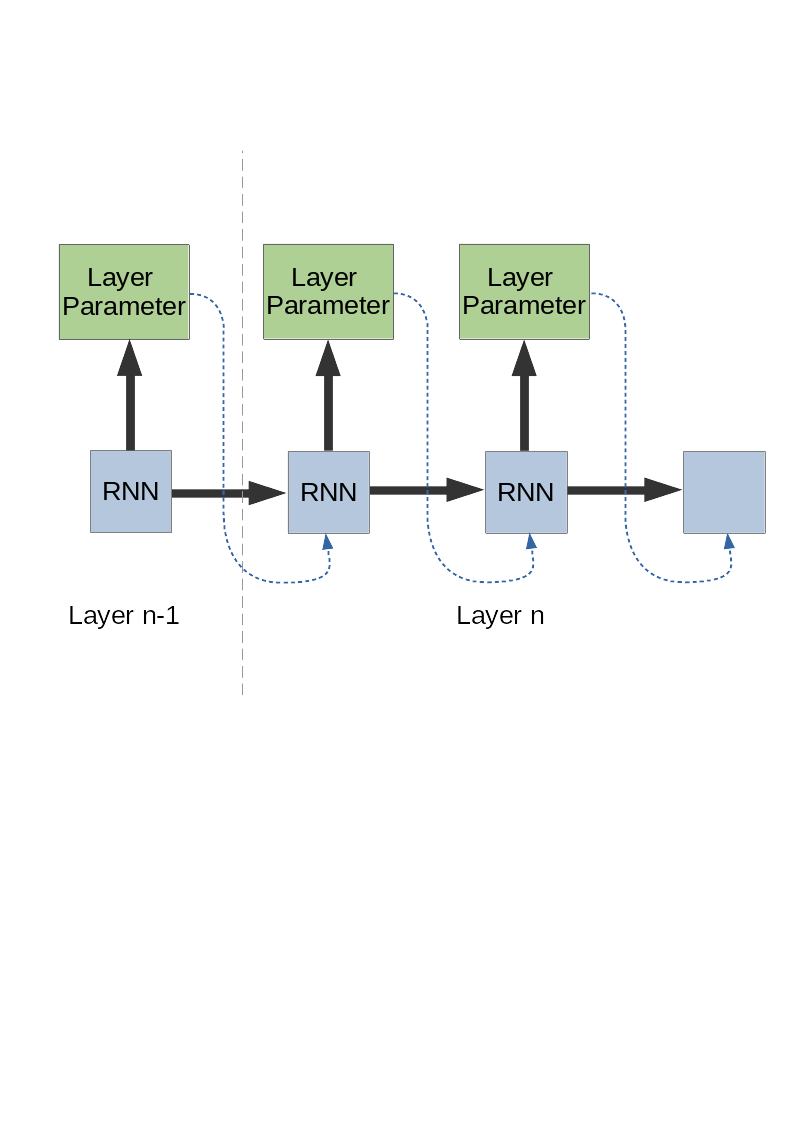
\includegraphics[trim=0 320 0 150 ,scale=0.3]{NAS-RL.png}
			\centering
			\caption{RNN controller in RL-NAS. The controller is a recurrent neural network (RNN), which at each time-step outputs a parameter for the current layer (i.e. number of node, filter size, dropout, ect). The number and order of these parameters is regular and the process simply repeats for each layer.   
			}
			\label{fig:RL}

	\end{figure}

  
	The extreme computational cost of RL-NAS lead to the development of Efficient Neural Architecture Search (ENAS). ENAS \cite{ENAS} was an expansion upon RL-NAS which was able to reduced the computational cost by a factor of more than 1000 and achieve slightly improved results setting a new SOTA on CIFAR-10. This was done by training a single acyclic graph within which the entire search-space was contained. This type of approach is now referred to as One-Shot NAS. This type of weight sharing can be considered an aggressive form of transfer learning. The key assumption here is that the performance of a network using a set of weights generated on a \textit{supernetwork} will correlate with true performance of the network. The importance of drop-out in the training of the supernetwork was shown in \cite{ENAS-T}. This method has also seen success recently with what is known as Few-Shot NAS \cite{fewshot}. In this approach the search space is split into a number of sub-\textit{supernetworks}. This allows the for a middle ground between One-Shot NAS and RL-NAS. 
	\par
	Another approach to this problem is to generate the network weights through the use of a \textit{HyperNetwork} \cite{hypernetworks}. The concept of a \textit{HyperNetwork} involves training a smaller network to generate the weights of a larger network. In particular this has interesting applications in RNNs where the weights can be generated dynamically at each time-step. SMASH \cite{smash} is an application of this method to the NAS problem which was able to achieve some success.  



%\section{Bi-Level/Gradient Descent}

%	[11] STNs - gradient descent for hyper-parameter optimisation

%	[53] Darts - gradient descent for cell architecture search  

%	Networks without training
    


\newpage
\section{Meta-Learning}

	Meta-learning has gained traction as a possible path away from the black-box perspective of hyper-parameter optimisation. This involves the application of machine learning to configuration selection. This has been implemented in various forms with success, such as a type of transfer learning in network embedding applications \cite{9}. This has also been implemented as an interface which allows experts to effectively warm start an auto-ML pipeline with knowledge of effective configurations for similarly structured problems\cite{29}. Another approach has been to train an agent via reinforcement learning to select configurations[28]. These applications of meta-learning are effective at reducing the convergence time however, rarely achieve significantly superior final performance than the methods they are supplementing.\cite{31}\cite{29}

%\printbibliography






\end{document}

